\chapter{Proposed Design \& Development}
\section{Design}
The project will be split into three views, the first, which will be similar to the wireframe in figure \ref{fig:view1} is a selection screen with a text area, where the user can select tags to search by inputting them.

\begin{figure}
	\caption[Screenshot of the Category Selection View]{Screenshot of the category selection view, where the user inputs the category of article they want to read, as well as their experience level.}
	\label{fig:view1}
	\begin{center}
	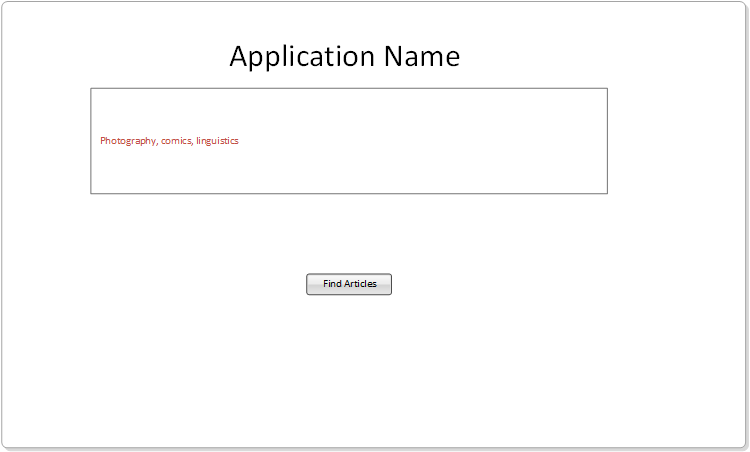
\includegraphics[width=\textwidth]{Graphics/View1}
	\end{center}
\end{figure}

Once the user inputs their preferred categories, the application takes those categories and finds relevant L2 articles by looking at articles on various sites, it then takes those articles and displays the title of each article, similar to view shown in figure \ref{fig:view2}

\begin{figure}
	\caption[Screenshot of the Article Selection View]{An example of the article selection view, here the user is shown a list of articles in their selected category as well as the difficulty rating for each article. They then go on to select an article from the list.}
	\label{fig:view2}
	\begin{center}
	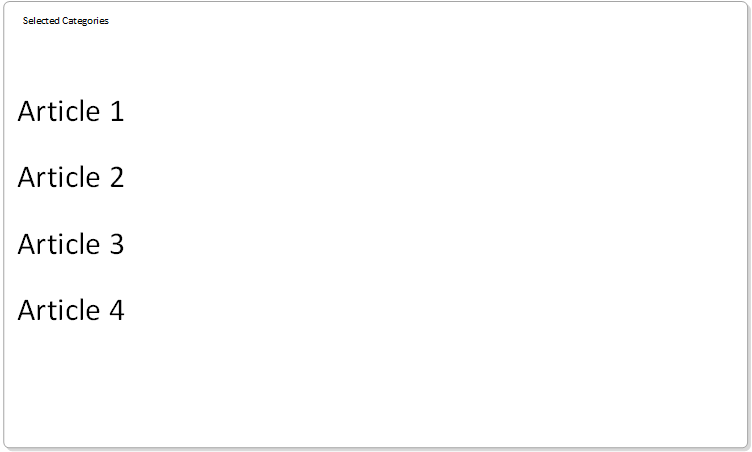
\includegraphics[width=\textwidth]{Graphics/View2}
\end{center}
\end{figure}

From the view shown in figure \ref{fig:view2} the user can select an article, once they do so, the application will download and parse the article, displaying it to the user, similar to the view in figure \ref{fig:view3}.

\begin{figure}
	\caption[Screenshot of the Article Reading View]{The article reading view, where the user can read the contents of their selected article. To the left of the article content is a button taking them back to article selection view and to the right is the gloss column, which contains a prompt telling the user click on articles. }
	\label{fig:view3}
	\begin{center}
	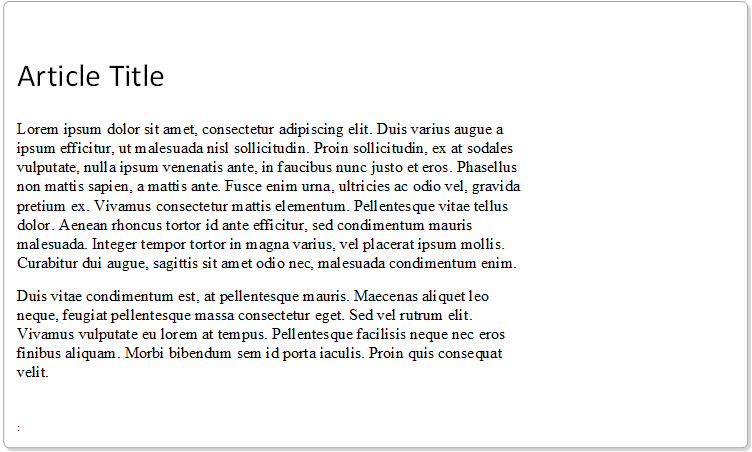
\includegraphics[width=0.7\textwidth]{Graphics/View3}
\end{center}
\end{figure}

from figure \ref{fig:view3} the user can select a word in the article, this action will send a request to the server for a gloss. The server will then look up translations of the word, along with grammatical information for the word, it will then serve the content, properly formatted, to the user, in a marginal gloss looking similar to the view in figure \ref{fig:view4}.

\begin{figure}
	\caption[Screenshot of the Article Reading View with Gloss]{Another screenshot of the article reading view, this time with a gloss entry in the margin.}
	\label{fig:view4}
	\begin{center}
	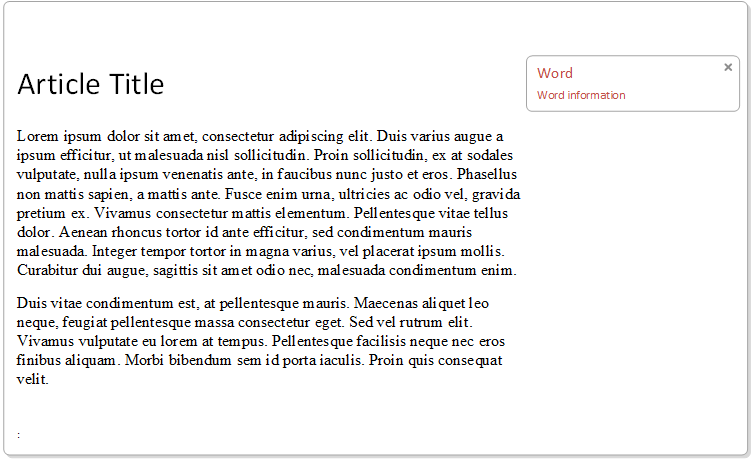
\includegraphics[width=\textwidth]{Graphics/View4}
\end{center}
\end{figure}

A marginal gloss in with multiple L1 translations and grammatical information as marginal glosses are effective \cite{abuseileek2008} and relatively easy to develop for. Multiple translations are being used to prevent the occurrence of an incorrect translation. 

The whole systems process is illustrated in figure \ref{fig:sf}.
	
\begin{figure}
	\caption{Wireframe Mockup of the Category Input View}
	\label{fig:sf}
	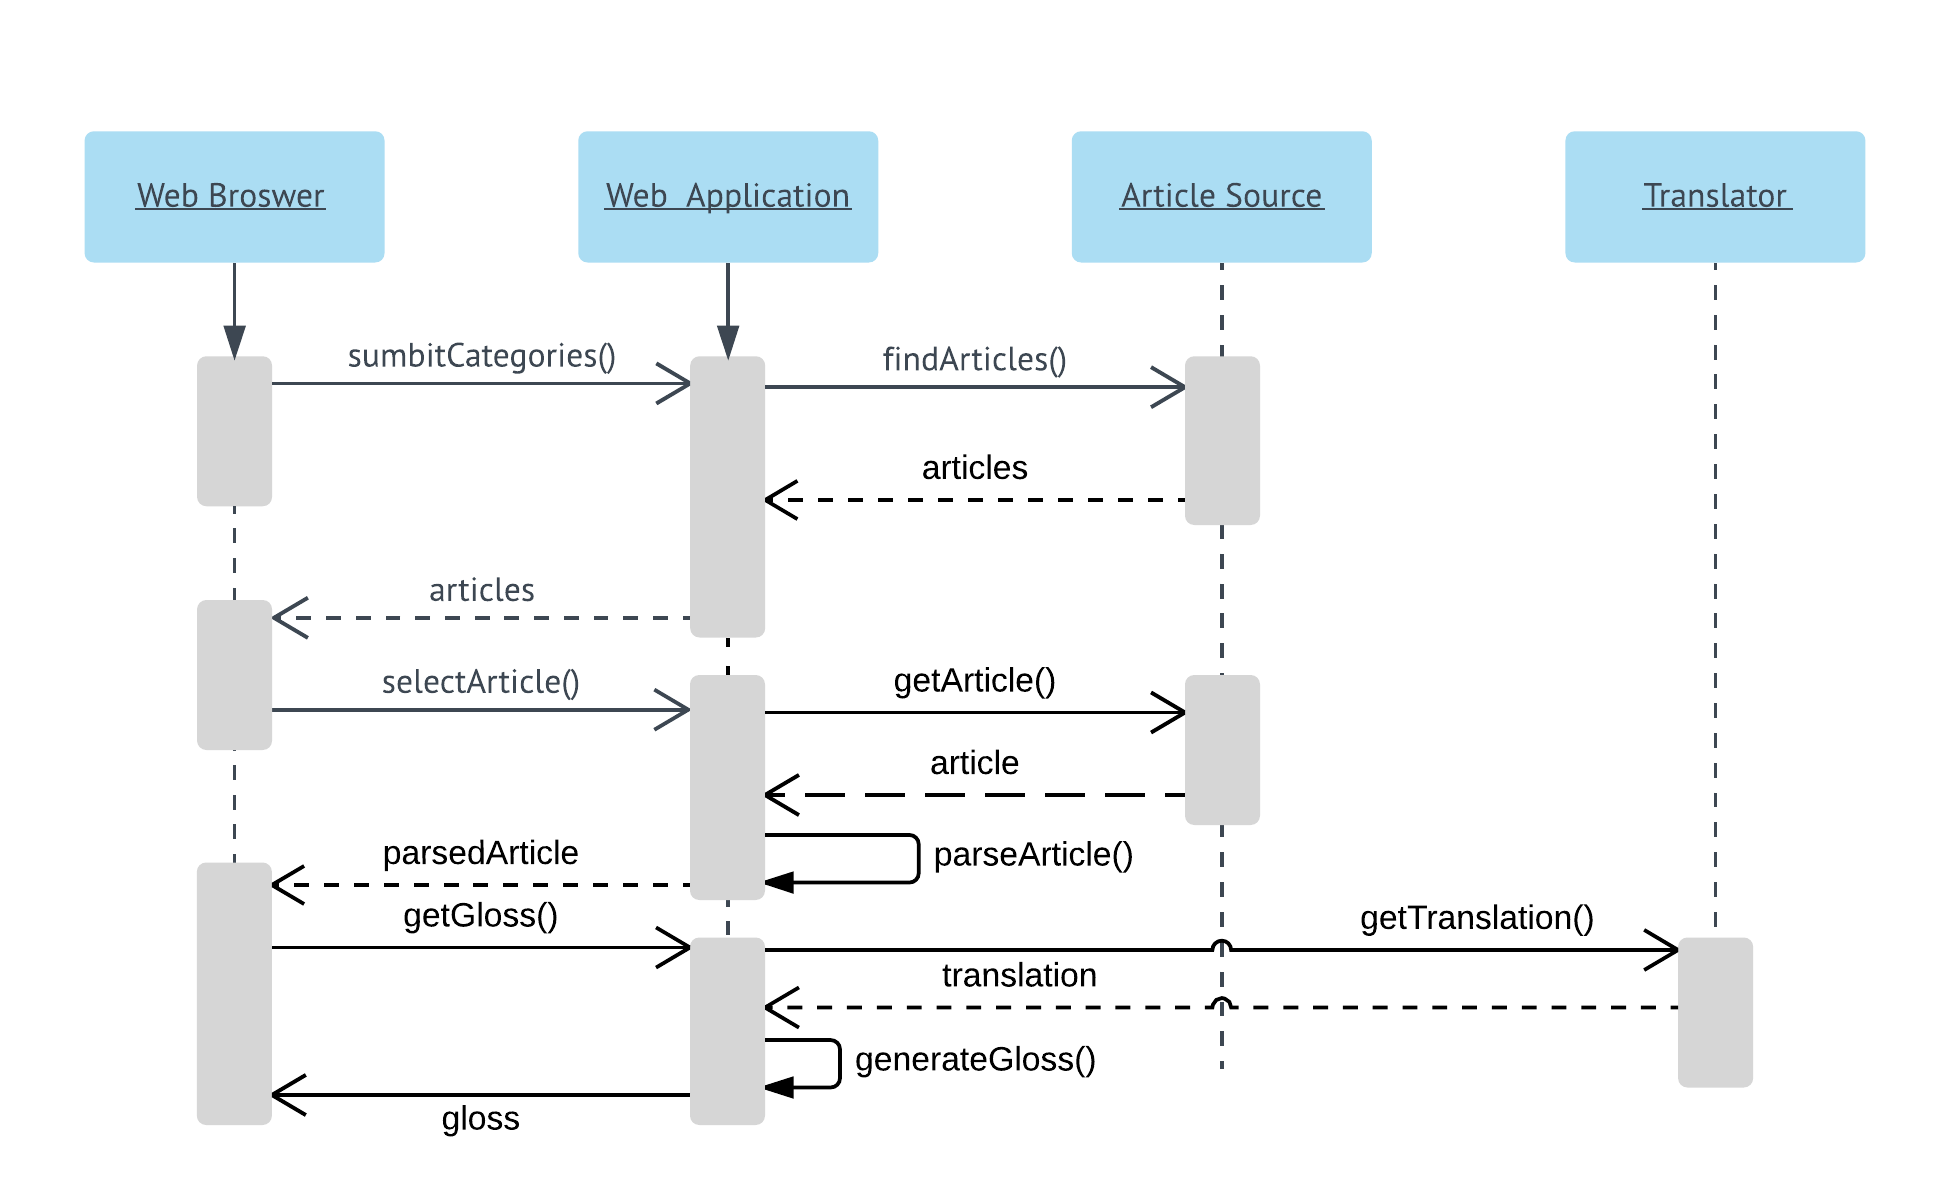
\includegraphics[width=\textwidth]{Graphics/SystemsFlow}
\end{figure}

\section{Development}

The plan is to develop the application using agile development structures using five sprints. Agile development was chosen because it allows for feedback to received on the project at weekly supervisor meetings, it also means that the development can be adjusted based on new ideas presented during the feedback session.

The five Sprints and their aims as as follows:
\begin{enumerate}
	\item \textbf{Translation Lookup}
	
	The aim of this sprint is to establish a valid method to retrieve single word translation and grammatical data.
	
	\item \textbf{Article Parsing \& Presentation}
	
	The aim of this sprint is develop a method for the parsing of articles and then to present them through a web browser
	
	\item \textbf{AJAX}
	
	The aim of this sprint is to develop the javscript code that will allow the gloss to display entries.
	
	\item \textbf{Recommender System}
	
	The aim of this sprint it to develop the recommender system that will suggest articles to the user. 
	
	\item \textbf{Advance Parsing}
	
	The aim of this sprint is to allow for advance parsing, such as parts of speech or the breaking up of German compound words into their component parts.
\end{enumerate}

These sprints were chosen as each of them represents a core development of a feature in the project. The order was chosen as it allows the project to reach minimum viable status as soon as possible (sprint 3). While leaving the most optional sprint until last.  

\section{Testing}
Preliminary testing will be done during and at the end of each sprint, this will allow the developer to test each part of the application, seeing if it works. Then the application as a whole will be tested. 

Once the five sprints have been completed, the application will have to be user-test to make sure it performs effectively. Users will test the application by using it, then answering a questionnaire about the application and their experiences using it. 

Splitting the testing into two main parts like this means that the testing of each indivual part will be completed in time for user testing, so the users will only ever been testing the complete application. Not performing user testing until the end of the project will mean that only one ethics approval will have to be submitted. 